\begin{figure}
    \centering
    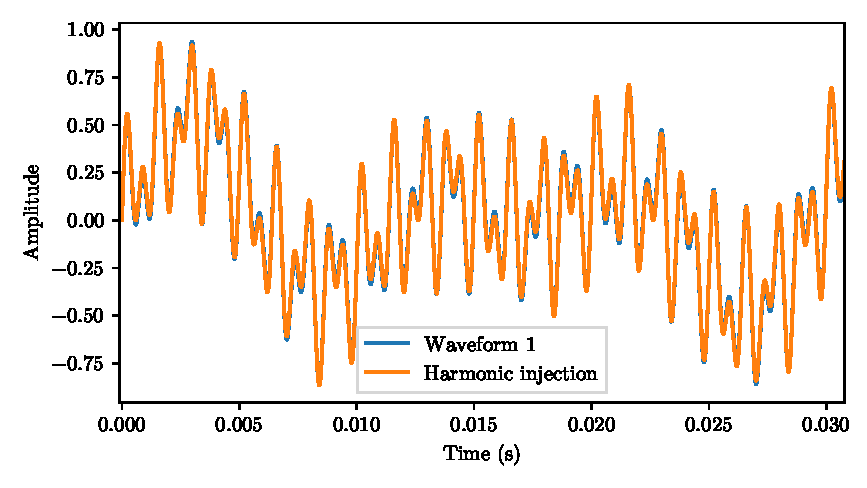
\includegraphics{Images/shaker/Figure_1.pdf}
    \caption{Waveform comparision of the shaker test.}
    \label{fig:shaker}
\end{figure}

\begin{figure}
    \centering
    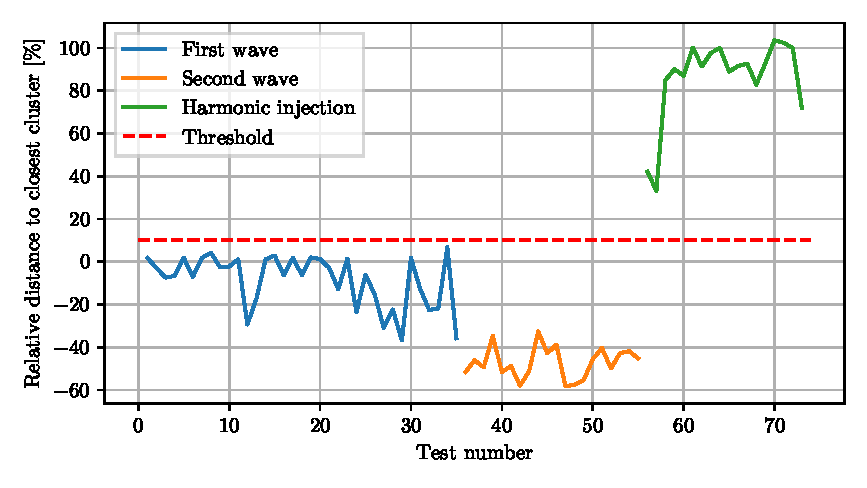
\includegraphics{Images/shaker/Results.pdf}
    \caption{Novelty detection result}
    \label{fig:shaker_results}
\end{figure}

\begin{figure}
    \centering
    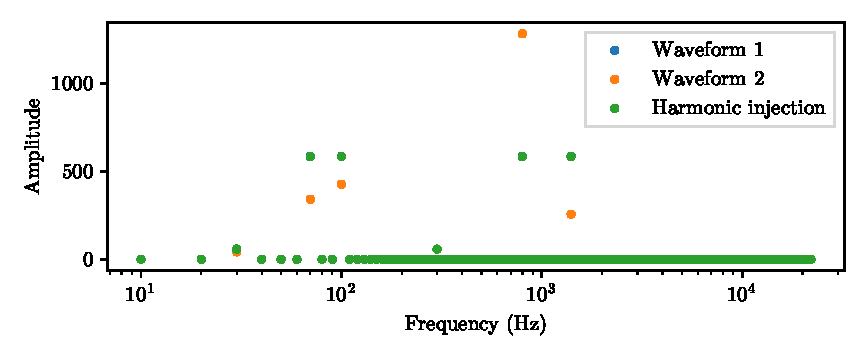
\includegraphics{Images/shaker/spectrum.pdf}
    \caption{Spectrum of the waveforms.}
    \label{fig:shaker_spectrum}
\end{figure}

\begin{table}[hbtp]
\centering
\begin{tabular}{|c|cccccc|}
\hline
\multirow{2}{*}{Signal} & \multicolumn{6}{c|}{Harmonic frequency {[}Hz{]}} \\
                        & 30     & 70     & 100   & 300   & 800   & 1400   \\ \hline
Wave 1                  & 0.1    & 1.0    & 1.0   & -     & 1.0   & 1.0    \\
Wave 2                  & 0.1    & 0.8    & 1.0   & -     & 3.0   & 0.6    \\
Test Wave               & 0.1    & 1.0    & 1.0   & 0.1   & 1.0   & 1.0    \\ \hline
\end{tabular}
\caption{Table of the harmonic coefficlients for the shaker test.}
\label{tab:shaker}
\end{table}

